\documentclass[a4paper,10pt]{report}

\topmargin -3cm
%\topskip0cm
%\footskip0cm
%\headsep0cm
\parindent0cm
\oddsidemargin -1cm
\evensidemargin -1cm
\headheight 3cm
\textheight 23cm
\textwidth 18cm

\author{Daniel W\"aber (4049590)}
\title{\"Ubung}

\usepackage{ucs}
\usepackage[utf8x]{inputenc}
\usepackage{german}
\usepackage{color}

\pagestyle{empty}
\usepackage{makeidx}
\usepackage{amsmath}
\usepackage{amsfonts}
\usepackage{amssymb,euscript}
\usepackage{dsfont}
\usepackage{listings}
\usepackage{enumerate}
\newfont{\Fr}{eufm10}
\newfont{\Sc}{eusm10}
\newfont{\Bb}{msbm10}
\newcommand{\limin}{\lim_{n\rightarrow\infty}}
\newcommand{\limix}{\lim_{x\rightarrow\infty}}
\newcommand{\limun}{\lim_{n\rightarrow -\infty}}
\newcommand{\limux}{\lim_{n\rightarrow -\infty}}
\newcommand{\limx}{\lim_{x\rightarrow x_0}}
\newcommand{\limh}{\lim_{h\rightarrow 0}}
\newcommand{\defi}{\paragraph{Definition:}}
\newcommand{\bew}{\paragraph{Beweis:}}
\newcommand{\satz}{\paragraph{Satz:}}
\newcommand{\bsp}{\paragraph{Beispiel:}}
\newcommand{\lemma}{\paragraph{Lemma:}}
\newcommand{\N}{\mathds{N}}
\newcommand{\Z}{\mathds{Z}}
\newcommand{\Q}{\mathds{Q}}
\newcommand{\R}{\mathds{R}}
\newcommand{\C}{\mathds{C}}
\newcommand{\K}{\mathds{K}}
\newcommand{\A}{\mathds{A}}
\newcommand{\qed}{$\hfill\blacksquare$}
\newcommand{\arsinh}{\operatorname{arsinh} }
\newcommand{\arcosh}{\operatorname{arcosh} }
\newcommand{\wP}{\mathcal{P} }
\newcommand{\gdw}{$\Leftrightarrow$}
\newcommand{\tf}{$\Rightarrow$}
\newcommand{\mgdw}{\Leftrightarrow}
\newcommand{\mtf}{\Rightarrow}
\newcommand{\Bild}{\text{Bild}}
\newcommand{\Kern}{\text{kern}}
\newcommand{\rg}{\text{rg}}
\newcommand{\deff}{\text{deff}}

\newcommand{\alphato}{\underset{\alpha}\to}
\newcommand{\betato}{\underset{\beta}\to}
\newcommand{\etato}{\underset{\eta}\to}
\newcommand{\ito}{\underset{i}\to}
\newcommand{\sto}{\underset{s}\to}
\newcommand{\kto}{\underset{k}\to}
\newcommand{\xto}{\underset{x}\to}

\usepackage{fancyhdr}
\pagestyle{fancy}
\lhead{Daniel Waeber\\Michael Kmoch}
\chead{"Ubungsblatt \nr\\\today}
\rhead{HA\\Tutor: Claudia Dieckmann}



\newcommand{\nr}{10}

\begin{document}
\section*{Aufgabe 1}
\begin{eqnarray}
-x_1 + x_2 \leq 0 &\Rightarrow& x_2 \leq x_1 \\
 x_1 - x_2 \leq 2 &\Rightarrow& x_2 \leq x_1 - 2 \\
 x_1 + x_2 \leq 2 &\Rightarrow& x_2 \leq -x_1 + 2 \\
-x_1 - x_2 \leq 0 &\Rightarrow& x_2 \geq -x_1 \\
x_1 \leq 3
\end{eqnarray}
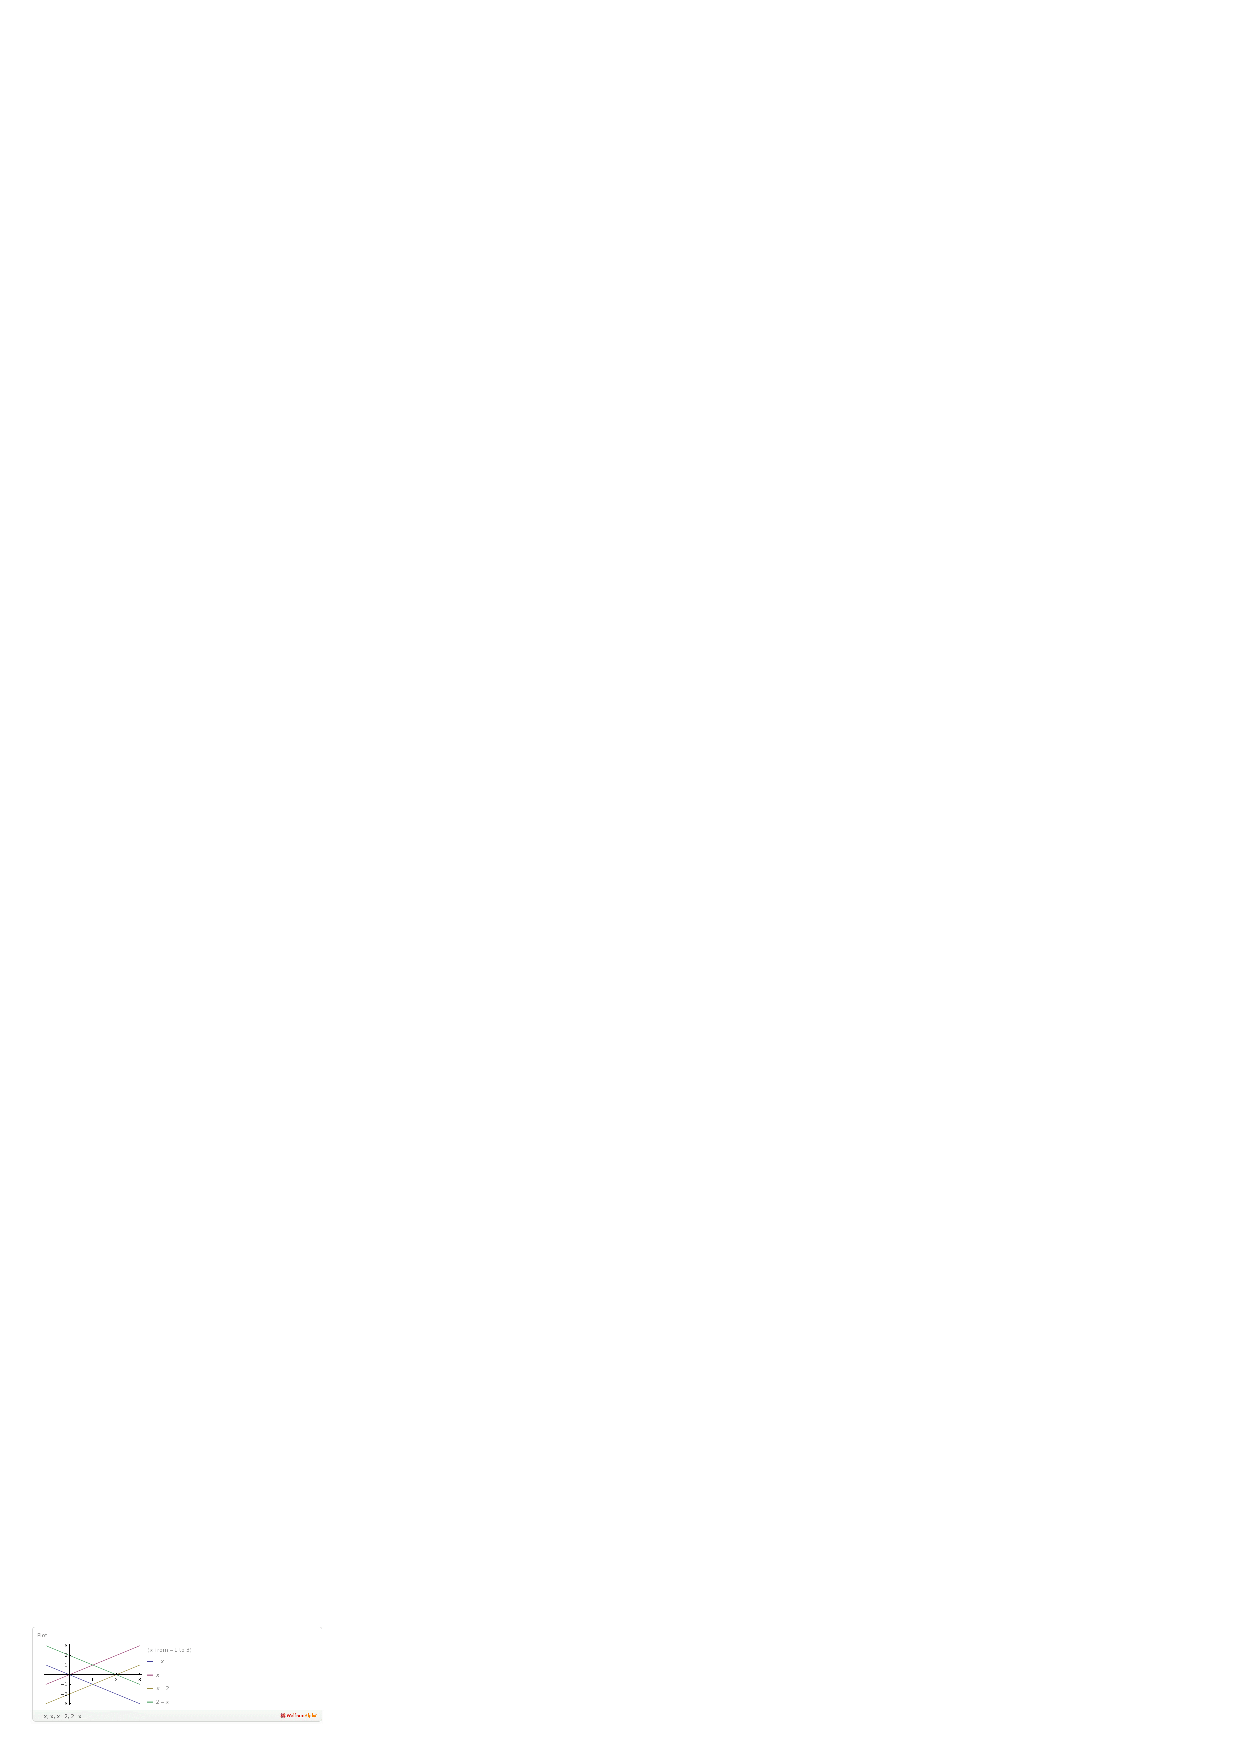
\includegraphics[width=\textwidth]{u10-plot}

\tf Loesungen inerhalb der umschlossenen Flaeche, als nur Richtung der Optimierung wichtig

\begin{enumerate}[a)]
\item $c =\left( \begin{matrix}1\\0\end{matrix} \right)$ 

 moeglichst weit links \tf Optimum bei $(0,0)$ mit Wert $0$

\item $c =\left( \begin{matrix}-3\\ 1\end{matrix} \right)$ 

 moeglichst weit in rechts unten \tf Optimum bei $(2,0)$ mit Wert $-3 \cdot 2 + 0 = -6$

\item $c =\left( \begin{matrix}-1\\ -1\end{matrix} \right)$ 

 Optimum auf gerade richts oben, c.B. bei $(1,1)$ mit Wert $-1-1 = -2$

\end{enumerate}

\section*{Aufgabe 2}
\begin{eqnarray}
s x_1 + t x_2 &\leq& 1\\
x_2 &\leq& -\frac{s}{t} x_1 + \frac{1}{t}\\
x_1 &\leq& -\frac{t}{s} x_2 + \frac{1}{s}
\end{eqnarray}

Eckpunkt bei $x_1$-Achse ($x_2=0$) bei $\frac{1}{s}$,
bei $x_2$-Achse ($x_1=0$) bei $\frac{1}{t}$.

Da die Reichtung der Optimierung $\left( \begin{matrix}1\\1\end{matrix} \right)$ ist,
und $x_1, x_2 \geq 0$ sein muessen, gilt

\begin{enumerate}[a)]
\item optimale Loesung, falls $x_1, x_2 > 0$
\item keine Loesung, falls $x_1, x_2 < 0$
\item unbeschrenkt, sonst
\end{enumerate}

\section*{Aufgabe 3}
\paragraph{a)}

\begin{eqnarray}
1 x_1 + 1 x_2 + 2 x_3 &\leq& 4 \\
2 x_1 + 0 x_2 + 3 x_3 &\leq& 5 \\
2 x_1 + 1 x_2 + 3 x_3 &\leq& 7
\end{eqnarray}

Einfuehrung der Schlupfwariablen und Zielfunktion als Gleichung:
\begin{eqnarray}
 1 x_1 + 1 x_2 + 2 x_3 + x_4 &=& 4 \\
 2 x_1 + 0 x_2 + 3 x_3 + x_5 &=& 5 \\
 2 x_1 + 1 x_2 + 3 x_3 + x_6 &=& 7 \\
 3 x_1 - 2 x_2 - 4 x_3       &=& z
\end{eqnarray}

Basis $x_4, x_5, x_6$:
\begin{eqnarray}
x_4 &=&  4 - 1 x_1 - 1 x_2 - 2 x_3 \\
x_5 &=&  5 - 2 x_1 + 0 x_2 - 3 x_3 \\
x_6 &=&  7 - 2 x_1 - 1 x_2 - 3 x_3 \\
z   &=&  0 - 3 x_1 - 2 x_2 - 4 x_3
\end{eqnarray}

Eintritsvariable $x_2$ \tf Austritt $x_4$:
\begin{eqnarray}
x_2 &=&  4 - 1 x_1 - 2 x_3 - 1 x_4 \\
x_5 &=&  5 - 2 x_1 + 3 x_3 + 0 x_4 \\
x_6 &=&  3 - 1 x_1 - 1 x_3 + 1 x_4 \\
z   &=& -8 - 1 x_1 + 2 x_4
\end{eqnarray}

Eintrittsvariable $x_1$ \tf Austritt $x_5$
\begin{eqnarray}
x_1 &=&  \frac{5}{2} + \frac{3}{2} x_3 + 0 x_4 - \frac{1}{2} x_5 \\
x_2 &=&  \frac{3}{2} - \frac{7}{2} x_3 - 1 x_4 + \frac{1}{2} x_5 \\
x_6 &=&  \frac{1}{2} - \frac{5}{2} x_3 + 1 x_4 + \frac{1}{2} x_5 \\
z   &=&-\frac{21}{2} - \frac{3}{2} x_3 + 2 x_4 + \frac{1}{2} x_5 \\
\end{eqnarray}

Eintrittsvariable $x_3$

\end{document}
